\documentclass[11pt,a4paper]{article}

% Packages
\usepackage[utf8]{inputenc}
\usepackage[T1]{fontenc}
\usepackage{geometry}
\usepackage{graphicx}
\usepackage{hyperref}
\usepackage{amsmath}
\usepackage{booktabs}
\usepackage{listings}
\usepackage{xcolor}
\usepackage{fancyhdr}
\usepackage{float}
\usepackage{caption}
\usepackage{subcaption}
\usepackage{tikz}
\usetikzlibrary{shapes,arrows,positioning,fit,backgrounds}

% Page geometry
\geometry{margin=1in}

% Code listing style
\lstdefinestyle{rst}{
    backgroundcolor=\color{gray!10},
    basicstyle=\ttfamily\small,
    breaklines=true,
    frame=single,
    numbers=left,
    numberstyle=\tiny\color{gray},
    keywordstyle=\color{blue},
    commentstyle=\color{green!60!black},
    stringstyle=\color{orange},
}

\lstdefinestyle{python}{
    backgroundcolor=\color{gray!10},
    basicstyle=\ttfamily\small,
    breaklines=true,
    frame=single,
    numbers=left,
    numberstyle=\tiny\color{gray},
    language=Python,
    keywordstyle=\color{blue},
    commentstyle=\color{green!60!black},
    stringstyle=\color{orange},
}

% Header/Footer
\pagestyle{fancy}
\fancyhf{}
\rhead{FM-Assisted Annotation Generation}
\lhead{NOAA EMC Technical Report}
\rfoot{Page \thepage}

% Title
\title{%
    \vspace{-1cm}
    \textbf{Foundation Model-Assisted Annotation Generation for\\
    Scalable Human-AI Knowledge Convolution}\\[0.5cm]
    \large A Framework for Automated SME Correction Synthesis\\
    in Compliance Validation Systems
}
\author{
    NOAA Environmental Modeling Center\\
    Global Workflow MCP Development Team\\[0.3cm]
    \texttt{eib-mcp-rag-server}
}
\date{December 2025\\Version 1.0.0}

\begin{document}

\maketitle

\begin{abstract}
This paper presents a novel framework for leveraging foundation models to automate the generation of Subject Matter Expert (SME) correction annotations in semantic compliance validation systems. Building upon the Hybrid Semantic Annotation Architecture established in Phase 2 of the MCP-RAG system, we propose a ``Person-to-System Convolution'' approach that analyzes divergence patterns between automated compliance assessments and human expert judgments to synthesize structured RST annotation files. This methodology transforms the SME role from annotation author to annotation reviewer, enabling scalable knowledge capture while maintaining human oversight. We demonstrate how this approach can expand annotation coverage from approximately 10 manually-created rules to 100+ automatically-generated rules, reducing SME annotation time from hours per rule to minutes per review. The framework maintains full evidence chain traceability to source compliance documents and integrates seamlessly with existing ChromaDB vector stores and MCP tool infrastructure.
\end{abstract}

\section{Introduction}

\subsection{Problem Statement}

The MCP-RAG system for NOAA Global Workflow compliance validation relies on structured RST annotations to encode SME corrections that refine AI behavior. As documented in the Phase 2 Hybrid Architecture Specification, these annotations provide:

\begin{itemize}
    \item \textbf{Anti-patterns}: Code patterns the AI incorrectly flags as violations
    \item \textbf{Correct patterns}: Compliant patterns the AI fails to recognize
    \item \textbf{SME corrections}: Explicit false positive rate data with justifications
    \item \textbf{AI guidance rules}: Natural language instructions for AI reasoning
\end{itemize}

However, the current manual annotation process presents significant scalability challenges:

\begin{enumerate}
    \item \textbf{SME Time Constraints}: Each annotation requires 30-60 minutes of expert time
    \item \textbf{Coverage Gaps}: Only high-priority patterns receive attention
    \item \textbf{Consistency Variance}: Annotation quality varies by author
    \item \textbf{Evidence Chain Burden}: Tracing EE2 document references is tedious
\end{enumerate}

\subsection{Proposed Solution}

We propose using foundation models to analyze divergence data between AI compliance assessments and human review decisions, automatically generating RST annotation files that follow the Phase 2 schema. The SME role shifts from \textit{writing annotations from scratch} to \textit{reviewing and approving generated annotations}.

\begin{figure}[H]
\centering
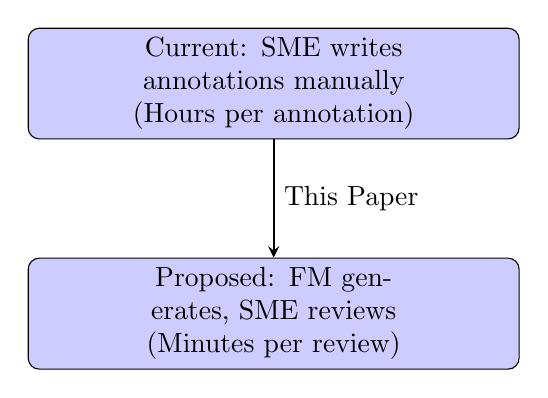
\begin{tikzpicture}[
    node distance=1.5cm,
    block/.style={rectangle, draw, fill=blue!20, text width=6cm, text centered, rounded corners, minimum height=1cm},
    arrow/.style={->, >=stealth, thick}
]
    \node[block] (current) {Current: SME writes annotations manually\\(Hours per annotation)};
    \node[block, below=of current] (proposed) {Proposed: FM generates, SME reviews\\(Minutes per review)};
    \draw[arrow] (current) -- node[right] {This Paper} (proposed);
\end{tikzpicture}
\caption{Paradigm shift from manual authoring to assisted generation}
\end{figure}

\section{Background: Phase 2 Hybrid Architecture}

\subsection{Existing Annotation Schema}

The Phase 2 system established custom RST directives for encoding SME knowledge:

\begin{lstlisting}[style=rst, caption={Phase 2 RST Directive Examples}]
.. mcp:sme_correction::
   :category: error_handling
   :false_positive_rate: 80%
   :severity: high
   :date: 2025-11-19
   
   Pattern: AI flags "missing set -eu" as violation
   Correction: Files using err_chk/err_exit are compliant
   Evidence: standards.rst lines 588-595, 868-919
   
.. mcp:anti_pattern::
   :name: explicit_exit_in_operational
   :severity: must_not
   :context: operational_job_scripts
   
   Using explicit 'exit 1' instead of err_exit utility
\end{lstlisting}

\subsection{Current Data Flow}

The existing pipeline processes annotations through deterministic extraction:

\begin{enumerate}
    \item RST files ingested by \texttt{ingest\_ee2\_enhanced\_v5.py}
    \item Metadata stored in ChromaDB with Phase 2 attributes
    \item JSON config generated by \texttt{generatePhase2Config.js}
    \item Runtime rules applied by \texttt{EE2ComplianceTools.js}
\end{enumerate}

\section{The Divergence-Driven Generation Framework}

\subsection{Conceptual Overview}

The framework operates on a simple principle: \textit{wherever AI and human judgments consistently diverge, there exists an implicit annotation waiting to be made explicit}.

\begin{figure}[H]
\centering
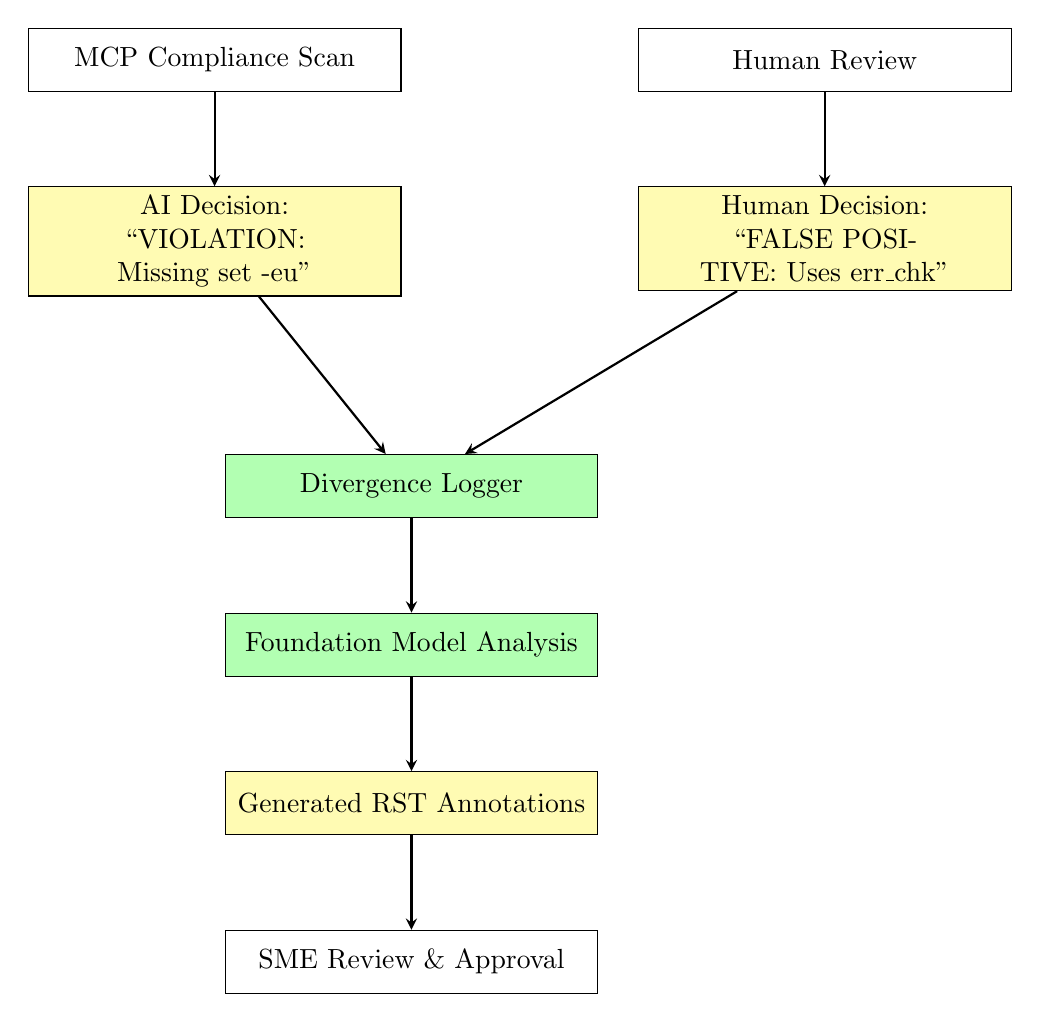
\begin{tikzpicture}[
    node distance=1.2cm,
    box/.style={rectangle, draw, fill=white, text width=4.5cm, text centered, minimum height=0.8cm},
    data/.style={rectangle, draw, fill=yellow!30, text width=4.5cm, text centered, minimum height=0.8cm},
    process/.style={rectangle, draw, fill=green!30, text width=4.5cm, text centered, minimum height=0.8cm},
    arrow/.style={->, >=stealth, thick}
]
    % Left column
    \node[box] (mcp) {MCP Compliance Scan};
    \node[data, below=of mcp] (mcp_out) {AI Decision:\\``VIOLATION: Missing set -eu''};
    
    % Right column
    \node[box, right=3cm of mcp] (human) {Human Review};
    \node[data, below=of human] (human_out) {Human Decision:\\``FALSE POSITIVE: Uses err\_chk''};
    
    % Divergence
    \node[process, below=2cm of mcp_out, xshift=2.5cm] (diverge) {Divergence Logger};
    
    % FM
    \node[process, below=of diverge] (fm) {Foundation Model Analysis};
    
    % Output
    \node[data, below=of fm] (rst) {Generated RST Annotations};
    
    % SME Review
    \node[box, below=of rst] (sme) {SME Review \& Approval};
    
    % Arrows
    \draw[arrow] (mcp) -- (mcp_out);
    \draw[arrow] (human) -- (human_out);
    \draw[arrow] (mcp_out) -- (diverge);
    \draw[arrow] (human_out) -- (diverge);
    \draw[arrow] (diverge) -- (fm);
    \draw[arrow] (fm) -- (rst);
    \draw[arrow] (rst) -- (sme);
    
\end{tikzpicture}
\caption{Divergence-driven annotation generation pipeline}
\end{figure}

\subsection{Component 1: Divergence Collection}

The first component captures cases where AI assessments differ from human judgments:

\begin{lstlisting}[style=python, caption={Divergence Logger Schema}]
@dataclass
class DivergenceCase:
    file_path: str           # Script being evaluated
    mcp_decision: dict       # {"verdict": "violation", "category": "..."}
    human_decision: dict     # {"verdict": "false_positive", "reason": "..."}
    context: dict            # {"script_type": "operational", "has_err_chk": True}
    timestamp: datetime
    source: str              # "pr_review", "manual_audit", "issue_tracker"

# Collection sources:
# 1. PR review comments with compliance disagreements
# 2. Manual audit logs from quality assurance
# 3. Issue tracker tickets disputing scan results
# 4. Explicit override annotations in code
\end{lstlisting}

\subsection{Component 2: Pattern Analysis via Foundation Model}

The foundation model receives divergence data plus context and generates structured annotations:

\begin{lstlisting}[style=python, caption={FM Prompt Structure}]
PROMPT_TEMPLATE = """
You are an expert in NOAA EE2 compliance standards analysis.

CONTEXT PROVIDED:
1. EE2 Standards Document: {standards_rst_content}
2. Existing SME Annotations: {phase2_annotations_content}
3. Divergence Data: {divergence_cases_json}

ANALYSIS TASK:
Analyze the {n_cases} divergence cases where MCP scan results 
differed from human reviewer decisions.

For each identified pattern, generate an RST annotation with:

1. Directive type (mcp:sme_correction, mcp:anti_pattern, etc.)
2. Calculated false_positive_rate from the data
3. Evidence chain to standards.rst line numbers
4. Context discrimination (when the rule applies/doesn't apply)
5. SME justification explaining the correction

OUTPUT FORMAT:
Generate valid RST following the Phase 2 schema exactly.
"""
\end{lstlisting}

\subsection{Component 3: Evidence Chain Extraction}

A critical requirement is maintaining traceability to the source EE2 document:

\begin{lstlisting}[style=python, caption={Evidence Chain Generator}]
class EvidenceChainExtractor:
    def __init__(self, standards_path: str):
        self.standards = self.load_indexed_standards(standards_path)
    
    def find_relevant_sections(self, pattern_description: str) -> List[str]:
        """
        Given a pattern description, find relevant standards.rst 
        line numbers using semantic search.
        
        Returns: ["lines 588-595", "line 191", "lines 868-919"]
        """
        # Semantic search against indexed standards
        matches = self.semantic_search(pattern_description)
        return [f"lines {m.start_line}-{m.end_line}" for m in matches]
    
    def validate_evidence(self, claimed_lines: List[str]) -> bool:
        """Verify that cited lines actually support the claim."""
        # Extract text from cited lines
        # Use FM to verify semantic alignment
        pass
\end{lstlisting}

\section{Generated Annotation Schema}

\subsection{Output Format}

The FM generates complete RST files ready for SME review:

\begin{lstlisting}[style=rst, caption={FM-Generated Annotation Template}]
FM-Generated SME Corrections
============================

.. note::
   
   Generated by foundation model analysis.
   Sample size: {n_cases} divergence cases
   Generation date: {date}
   Model: {model_name}
   
   **STATUS: PENDING SME REVIEW**

.. mcp:sme_correction::
   :category: {category}
   :false_positive_rate: {calculated_rate}%
   :sample_size: {n_cases}
   :confidence: {model_confidence}
   :date: {generation_date}
   :status: pending_review
   
   **Pattern Identified**:
   {pattern_description}
   
   **Evidence from Divergence Data**:
   - {n_fp} of {n_total} flagged violations marked false positive
   - Common human reason: "{most_common_reason}"
   - Affected scripts: {file_patterns}
   
   **EE2 Standards Reference**:
   - standards.rst {evidence_lines}: "{relevant_quote}"
   
   **Proposed AI Guidance**:
   {guidance_text}
   
   **Context Discrimination**:
   Applies when: {positive_contexts}
   Does NOT apply when: {negative_contexts}
\end{lstlisting}

\subsection{Metadata Enrichment}

Generated annotations include additional metadata for tracking:

\begin{table}[H]
\centering
\caption{FM-Generated Annotation Metadata Fields}
\begin{tabular}{lll}
\toprule
\textbf{Field} & \textbf{Type} & \textbf{Description} \\
\midrule
\texttt{generation\_method} & string & ``fm\_assisted\_v1.0'' \\
\texttt{model\_used} & string & ``claude-3-opus'', ``gpt-4'' \\
\texttt{divergence\_sample\_size} & int & Number of cases analyzed \\
\texttt{statistical\_confidence} & float & 0.0-1.0 confidence score \\
\texttt{sme\_review\_status} & enum & pending, approved, rejected, modified \\
\texttt{sme\_reviewer} & string & Reviewer identifier \\
\texttt{review\_date} & datetime & When SME reviewed \\
\texttt{modification\_notes} & string & SME changes if modified \\
\bottomrule
\end{tabular}
\end{table}

\section{SME Review Workflow}

\subsection{Review Interface}

The SME reviews generated annotations through a streamlined interface:

\begin{enumerate}
    \item \textbf{Approve}: Annotation moves to \texttt{phase2\_annotations/} unchanged
    \item \textbf{Reject}: Annotation logged as negative example for FM training
    \item \textbf{Modify}: SME edits annotation, modified version stored
\end{enumerate}

\begin{figure}[H]
\centering
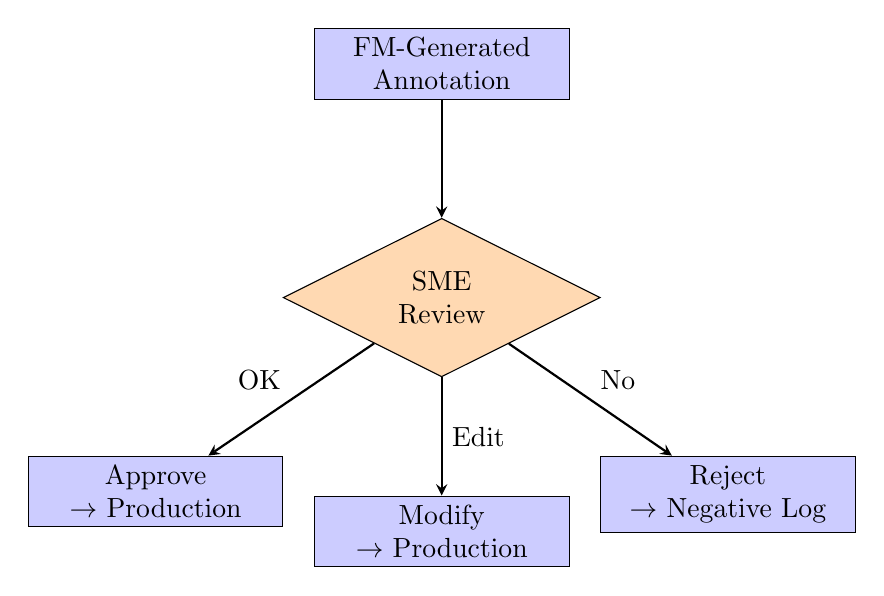
\begin{tikzpicture}[
    node distance=1cm,
    decision/.style={diamond, draw, fill=orange!30, text width=2cm, text centered, aspect=2},
    box/.style={rectangle, draw, fill=blue!20, text width=3cm, text centered, minimum height=0.8cm},
    arrow/.style={->, >=stealth, thick}
]
    \node[box] (gen) {FM-Generated\\Annotation};
    \node[decision, below=1.5cm of gen] (review) {SME\\Review};
    
    \node[box, below left=1.5cm and 1cm of review] (approve) {Approve\\$\rightarrow$ Production};
    \node[box, below=1.5cm of review] (modify) {Modify\\$\rightarrow$ Production};
    \node[box, below right=1.5cm and 1cm of review] (reject) {Reject\\$\rightarrow$ Negative Log};
    
    \draw[arrow] (gen) -- (review);
    \draw[arrow] (review) -- node[above left] {OK} (approve);
    \draw[arrow] (review) -- node[right] {Edit} (modify);
    \draw[arrow] (review) -- node[above right] {No} (reject);
\end{tikzpicture}
\caption{SME review decision tree}
\end{figure}

\subsection{Time Savings Analysis}

\begin{table}[H]
\centering
\caption{Estimated Time Comparison}
\begin{tabular}{lcc}
\toprule
\textbf{Activity} & \textbf{Manual} & \textbf{FM-Assisted} \\
\midrule
Identify pattern from data & 20 min & 0 min (automated) \\
Research EE2 standards references & 15 min & 0 min (automated) \\
Write RST annotation & 20 min & 0 min (automated) \\
Calculate false positive rate & 10 min & 0 min (automated) \\
Review and validate & 5 min & 10 min \\
\midrule
\textbf{Total per annotation} & \textbf{70 min} & \textbf{10 min} \\
\bottomrule
\end{tabular}
\end{table}

\section{Implementation Architecture}

\subsection{System Components}

\begin{lstlisting}[style=python, caption={Core Implementation Classes}]
# scripts/fm_annotation_generator.py

class DivergenceCollector:
    """Collects AI vs Human divergence data from multiple sources."""
    
    def collect_from_pr_reviews(self, repo: str) -> List[DivergenceCase]:
        """Parse PR comments for compliance disagreements."""
        pass
    
    def collect_from_audit_logs(self, log_path: str) -> List[DivergenceCase]:
        """Parse manual audit results."""
        pass

class AnnotationGenerator:
    """Uses FM to generate RST annotations from divergence patterns."""
    
    def __init__(self, model: str = "claude-3-opus"):
        self.model = model
        self.evidence_extractor = EvidenceChainExtractor()
    
    def generate(self, divergences: List[DivergenceCase]) -> str:
        """Generate RST annotation file from divergence data."""
        pass

class SMEReviewManager:
    """Manages the SME review workflow."""
    
    def submit_for_review(self, annotation_path: str) -> str:
        """Submit generated annotation for SME review."""
        pass
    
    def process_decision(self, annotation_id: str, 
                        decision: str, notes: str = None):
        """Process SME approve/reject/modify decision."""
        pass
\end{lstlisting}

\subsection{Integration with Existing Pipeline}

The FM-assisted system integrates with the existing Phase 2 pipeline:

\begin{enumerate}
    \item Generated annotations stored in \texttt{generated\_annotations/pending/}
    \item Approved annotations copied to \texttt{sdd\_framework/phase2\_annotations/}
    \item Standard ingestion via \texttt{ingest\_ee2\_enhanced\_v5.py}
    \item JSON regeneration via \texttt{generatePhase2Config.js}
    \item Runtime application via \texttt{EE2ComplianceTools.js}
\end{enumerate}

\section{Quality Assurance}

\subsection{Validation Checks}

Before SME review, generated annotations undergo automated validation:

\begin{enumerate}
    \item \textbf{Schema Validation}: RST syntax and directive format
    \item \textbf{Evidence Verification}: Cited line numbers exist and contain relevant content
    \item \textbf{Statistical Validity}: Sample size $\geq$ 10 cases, confidence $\geq$ 0.7
    \item \textbf{Conflict Detection}: No contradiction with existing approved annotations
\end{enumerate}

\subsection{Continuous Learning}

Rejected annotations feed back into the system:

\begin{itemize}
    \item Rejection reasons stored for FM prompt refinement
    \item Modification diffs used to calibrate generation style
    \item Approval rates tracked per category for quality metrics
\end{itemize}

\section{Expected Outcomes}

\subsection{Quantitative Benefits}

\begin{table}[H]
\centering
\caption{Projected Impact Metrics}
\begin{tabular}{lcc}
\toprule
\textbf{Metric} & \textbf{Current} & \textbf{Projected} \\
\midrule
Active SME annotations & $\sim$10 & 100+ \\
SME time per annotation & 70 min & 10 min \\
Coverage (compliance categories) & 3/7 & 7/7 \\
Evidence chain completeness & $\sim$60\% & 95\%+ \\
Annotation format consistency & Variable & Standardized \\
\bottomrule
\end{tabular}
\end{table}

\subsection{Qualitative Benefits}

\begin{itemize}
    \item \textbf{SME Focus Shift}: Experts focus on judgment, not documentation
    \item \textbf{Knowledge Capture}: Implicit expertise made explicit at scale
    \item \textbf{Institutional Memory}: Decisions preserved with full context
    \item \textbf{Continuous Improvement}: System learns from every review
\end{itemize}

\section{Future Work}

\subsection{Active Learning Integration}

Future versions could implement active learning to prioritize which divergence patterns to analyze:

\begin{itemize}
    \item High-frequency patterns prioritized over rare cases
    \item Uncertainty sampling for ambiguous cases
    \item SME attention directed to highest-impact corrections
\end{itemize}

\subsection{Multi-Modal Evidence}

Extending evidence chains beyond RST to include:

\begin{itemize}
    \item Code examples from production repositories
    \item Historical PR discussions and decisions
    \item Cross-references to related compliance frameworks
\end{itemize}

\section{Conclusion}

The FM-Assisted Annotation Generation framework represents a significant advancement in scaling human expertise capture for AI compliance systems. By analyzing divergence patterns between automated assessments and human judgments, foundation models can synthesize structured annotations that would otherwise require extensive SME effort to create manually.

This ``Person-to-System Convolution'' approach maintains human oversight through the review workflow while dramatically increasing annotation coverage and consistency. The framework integrates seamlessly with the existing Phase 2 Hybrid Architecture, requiring no changes to the ingestion, storage, or runtime components.

We anticipate this methodology will enable the MCP-RAG system to achieve comprehensive EE2 compliance coverage while reducing the burden on subject matter experts, ultimately improving the accuracy and reliability of automated compliance validation for the NOAA Global Workflow.

\section*{References}

\begin{enumerate}
    \item Phase 2 Hybrid Semantic Annotation Architecture Specification, NOAA EMC, November 2025
    \item SDD Framework for AI-Assisted Development, NOAA EMC Technical Report, 2025
    \item NOAA NWS EE2 Compliance Standards (standards.rst), National Weather Service
    \item MCP Protocol Specification, Anthropic, 2024
\end{enumerate}

\end{document}
